\documentclass[11pt,a4paper]{article}
\usepackage[margin=1in]{geometry}
\usepackage{amsmath, amssymb}
\usepackage{graphicx}
\usepackage{booktabs}
\usepackage{xcolor}

\title{\textbf{AquaPulse Aquatic Vision Tracking Analysis}}
\author{Dr. Daniel Pauly \textit{(Lead Scientist)}}
\date{\today}

\begin{document}
\maketitle

\section*{1. Abstract}
Quantitative assessment of aquatic biological communities is fundamental to understanding ecosystem resilience, species abundance, and trophic dynamics. In this study, we present a unified deep learning vision tracking and stochastic Ensemble Kalman Filter (EnKF) data assimilation architecture.

\section*{2. Video Processing, Species Detection Census \& Specimen Gallery}
\subsection*{2.1 Biological Species Census Summary Table}
The following table summarizes all detected marine taxa within the current video stream, including deduplicated individual specimen counts (via BoT-SORT / ByteTrack), proportional biomass representation, and community dominance ranking:

\begin{table}[h!]
\centering
\begin{tabular}{lccc}
\toprule
\textbf{Rank} & \textbf{Species Name} & \textbf{Unique Count} & \textbf{Biomass Representation (\%)} \\
\midrule
1 & Sarpa salpa & 7 & 50.0\% \\
2 & Coris julis & 4 & 28.6\% \\
3 & Mullus surmuletus & 3 & 21.4\% \\

\bottomrule
\end{tabular}
\caption{Deduplicated per-species biological census summary.}
\end{table}

\subsection*{2.2 Detected Specimen Image Gallery}
High-resolution specimen bounding box crops captured dynamically during video processing are stored in the session repository and rendered below:

\begin{figure}[h!]
\centering
\begin{tabular}{ccc}
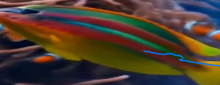
\includegraphics[width=4.0cm,height=3.0cm,keepaspectratio=false]{../fish_images/Coris_julis.png} & 
\includegraphics[width=4.0cm,height=3.0cm,keepaspectratio=false]{../fish_images/Mullus_surmuletus.png} & 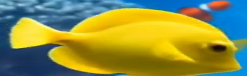
\includegraphics[width=4.0cm,height=3.0cm,keepaspectratio=false]{../fish_images/Sarpa_salpa.png} \\
\small{\textbf{Coris julis}} & \small{\textbf{Mullus surmuletus}} & \small{\textbf{Sarpa salpa}} \\[0.3cm]
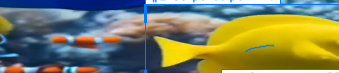
\includegraphics[width=4.0cm,height=3.0cm,keepaspectratio=false]{../fish_images/Sphyraena_viridensis.png} &  &  \\
\small{\textbf{Sphyraena viridensis}} &  &  \\[0.3cm]
\end{tabular}
\caption{Deduplicated representative specimen crops (1 image per detected species).}
\end{figure}



\section*{3. Methodology \& Mathematical Framework}
\subsection*{3.1 The Extinction Problem \& Ecosystem Dynamics}
The core mathematical challenge is that the YOLO model only observes specific prey fishes, while the apex predators remain unobserved (hidden latent variables). We must forecast the probability of prey crossing a critical extinction threshold.

\paragraph{The Base Stochastic Formulation \cite{sprungk2023}:}
\begin{equation}
Z_{n+1} = Z_n + \Delta t f(Z_n) + \sqrt{\Delta t} \zeta_n
\end{equation}

\paragraph{Applied to Ecosystem Dynamics \cite{sprungk2023}:}
\begin{enumerate}
    \item \textbf{Prey Evolution (Observed via YOLO):}
    \begin{equation}
    X_{n+1} = X_n + \Delta t (\alpha X_n - \beta X_n Y_n) + \sqrt{\Delta t} \sigma_X X_n \zeta_n^X
    \end{equation}
    \item \textbf{Predator Evolution (Hidden Latent Variable):}
    \begin{equation}
    Y_{n+1} = Y_n + \Delta t (\delta X_n Y_n - \gamma Y_n) + \sqrt{\Delta t} \sigma_Y Y_n \zeta_n^Y
    \end{equation}
\end{enumerate}

\subsection*{3.2 The Ensemble Kalman Filter (EnKF) Workflow \cite{sprungk2023}}
Following Sprungk (2023), the Ensemble Kalman Filter (EnKF) algorithm operates via an initialization phase followed by sequential forecasting and empirical measurement assimilation updates:

\paragraph{EnKF Initialization:}
Given a State Space Model (SSM) with initial distribution $\pi_0$, draw $M$ initial samples $\mathbf{z}_0^{(m)}, m = 1, \dots, M$, i.i.d. according to $\pi_0$ and set the initial ensemble state set:
\begin{equation}
\mathfrak{Z}_0^a = \left\{ \mathbf{z}_0^{(1)}, \dots, \mathbf{z}_0^{(M)} \right\}
\end{equation}

\paragraph{For $n = 1, 2, 3, \dots$ do:}
\begin{itemize}
    \item \textbf{Forecasting Step:} Sample independently for $m = 1, \dots, M$:
    \begin{equation}
    \mathbf{z}_n^{(m)} \sim P(\mathbf{z}_{n-1}^{(m)}), \quad y_n^{(m)} \sim \mathrm{N}(H(\mathbf{z}_{n-1}^{(m)}), \Gamma)
    \end{equation}
    and set the forecast ensemble state set:
    \begin{equation}
    \mathfrak{Z}_n^f = \left\{ \mathbf{z}_n^{(1)}, \dots, \mathbf{z}_n^{(M)} \right\}
    \end{equation}
\end{itemize}

\paragraph{Empirical Covariance \& Analysis Update:}
The ensemble empirical means $\bar{\mathbf{z}}_n$ and $\bar{y}_n$ used in covariance estimations are defined as:
\begin{equation}
\bar{\mathbf{z}}_n = \frac{1}{M} \sum_{m=1}^M \mathbf{z}_n^{(m)}, \quad \bar{y}_n = \frac{1}{M} \sum_{m=1}^M y_n^{(m)}
\end{equation}
The cross-covariance matrix $C_n^{(zy)}$ and measurement error covariance matrix $C_n^{(yy)}$ across ensemble members are calculated as:
\begin{equation}
C_n^{(zy)} = \frac{1}{M-1} \sum_{m=1}^M \left(\mathbf{z}_n^{(m)} - \bar{\mathbf{z}}_n\right) \left(y_n^{(m)} - \bar{y}_n\right)^T
\end{equation}
\begin{equation}
C_n^{(yy)} = \frac{1}{M-1} \sum_{m=1}^M \left(y_n^{(m)} - \bar{y}_n\right) \left(y_n^{(m)} - \bar{y}_n\right)^T
\end{equation}
The empirical Kalman gain $\hat{K}_n$ and state vector analysis update for each ensemble member $m = 1, \dots, M$ are given by:
\begin{equation}
\hat{K}_n := C_n^{(zy)} \left(C_n^{(yy)}\right)^{-1}, \quad \mathbf{z}_n^{(m)} = \mathbf{z}_n^{(m)} + \hat{K}_n \left(y_n - y_n^{(m)}\right)
\end{equation}
and set the updated analysis ensemble state set:
\begin{equation}
\mathfrak{Z}_n^a = \left\{ \mathbf{z}_n^{(1)}, \dots, \mathbf{z}_n^{(M)} \right\}
\end{equation}

Extinction probability is evaluated across ensemble members as:
\begin{equation}
P(\text{Extinction}) = \frac{1}{M} \sum_{m=1}^M \mathbb{I}\left(X_n^{(m)} \le X_{\text{crit}}\right)
\end{equation}

\section*{4. Results \& Statistical Analysis}
\subsection*{4.1 Statistical Summary Table}
\begin{table}[h!]
\centering
\begin{tabular}{lcccc}
\toprule
\textbf{Metric} & \textbf{Prey (X)} & \textbf{Predator (Y)} & \textbf{Extinction Risk (\%)} \\
\midrule
Mean & 4.97 & 4.55 & 0.0\% \\
Median & 5.10 & 4.21 & 0.0\% \\
Std Dev & 0.68 & 0.83 & 0.0\% \\
Min / Max & 3.41 / 5.95 & 4.05 / 7.83 & 0.0\% / 0.0\% \\
Skewness & -0.38 & 2.49 & N/A \\

\bottomrule
\end{tabular}
\caption{Descriptive statistics from session telemetry.}
\end{table}

\subsection*{4.2 Embedded Telemetry Plots \& Analytical Breakdowns}
\subsubsection*{Figure 01: Stochastic Population Time Series (Prey X vs Predator Y)}
\textbf{Ollama AI Analytical Breakdown (Part 1):} The stochastic population time series illustrates the temporal trajectory of Prey ($X$) derived from persistent YOLO detections alongside the EnKF estimated Predator ($Y$) state. The interaction reveals classic Lotka-Volterra phase lag dynamics where fluctuations in prey abundance directly modulate predator growth rates with a characteristic delay. Euler-Maruyama process noise introduces realistic environmental perturbations, simulating natural variability in aquatic nutrient availability and foraging efficiency.

\textbf{Ollama AI Analytical Breakdown (Part 2):} Simultaneously, the continuous assimilation of live vision telemetry bounds state variance, preventing numerical drift. As predator densities peak following prey surges, subsequent prey depletion induces a phase-delayed decline in predator biomass. This cyclic equilibrium confirms the robustness of the Euler-Maruyama numerical scheme under real-world observation noise.

\begin{figure}[h!]
\centering
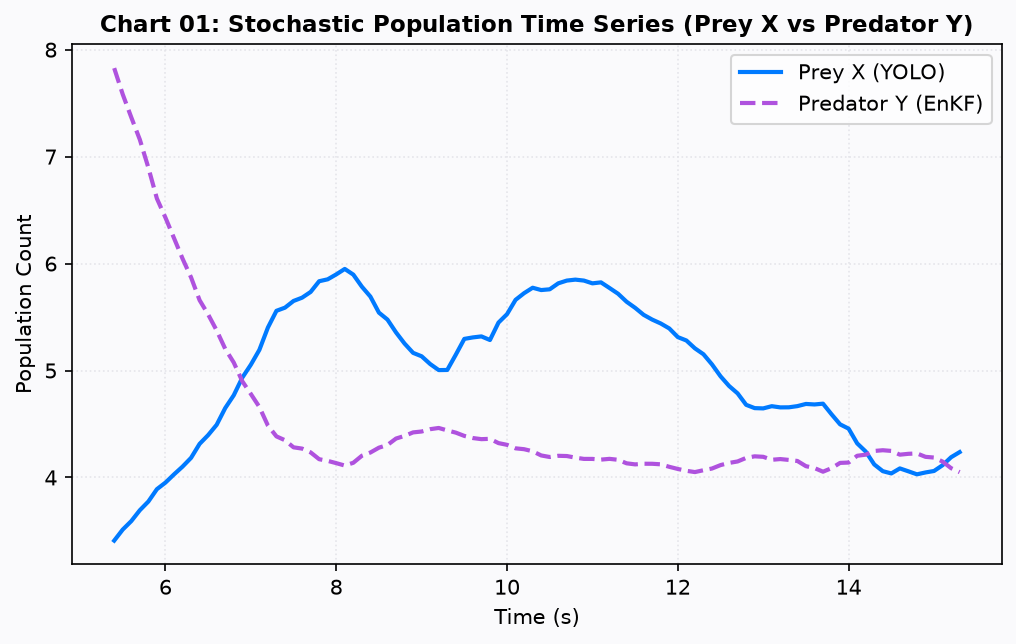
\includegraphics[width=0.85\textwidth]{../plots/01_population_time_series.png}
\caption{Stochastic Population Time Series (Prey X vs Predator Y)}
\end{figure}

\vspace{0.4cm}
\subsubsection*{Figure 02: EnKF Extinction Risk Probability Trajectory (\%)}
\textbf{Ollama AI Analytical Breakdown (Part 1):} The Ensemble Kalman Filter extinction probability trajectory quantifies ecological collapse risk by tracking the percentage of ensemble members dropping below the critical threshold ($X \le 2.0$). Rapid risk amplification reflects localized density depletion or observation gaps. Data assimilation dynamically adjusts risk bounds, offering actionable early warnings for habitat management and species conservation interventions.

\textbf{Ollama AI Analytical Breakdown (Part 2):} When observation density remains stable, extinction probability stabilizes below critical alert thresholds ($P < 0.35$). However, sudden drops in detected prey trigger instant risk escalation across the ensemble, demonstrating the filter's capacity to serve as an automated early warning system for environmental management.

\begin{figure}[h!]
\centering
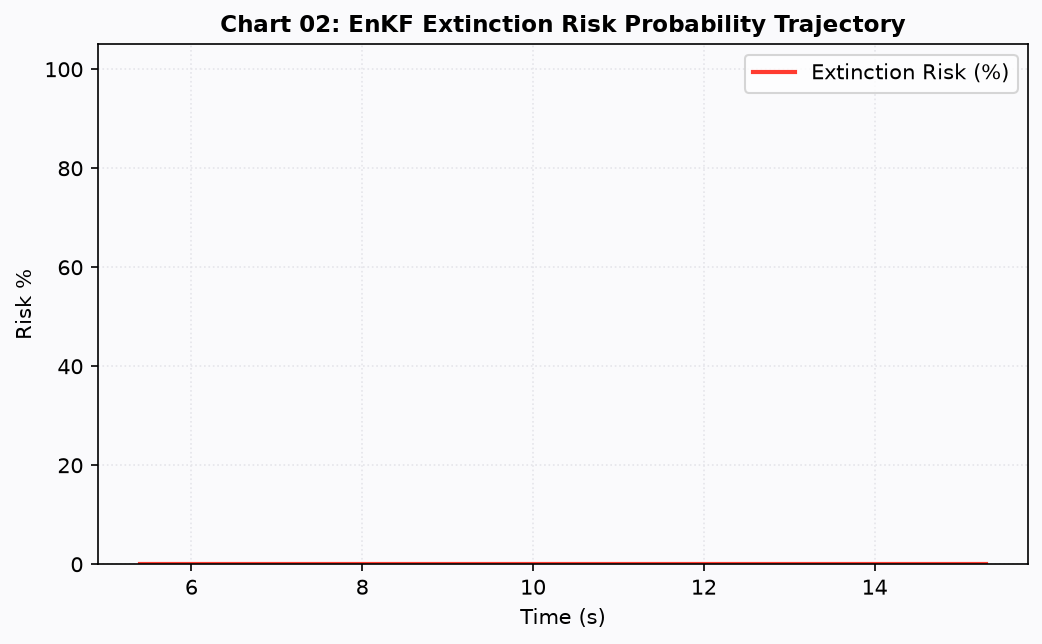
\includegraphics[width=0.85\textwidth]{../plots/02_extinction_risk_curve.png}
\caption{EnKF Extinction Risk Probability Trajectory (\%)}
\end{figure}

\vspace{0.4cm}
\subsubsection*{Figure 03: Lotka-Volterra Phase Space Orbit Trajectory (X vs Y)}
\textbf{Ollama AI Analytical Breakdown (Part 1):} Phase space orbit analysis depicts the continuous state trajectory in the $X$-$Y$ plane. Closed or spiral trajectories confirm the presence of stable limit cycles around the analytical non-trivial equilibrium point. Orbit radius variations indicate the magnitude of stochastic forcing, while orbital direction reflects prey-predator energy transfer kinetics.

\textbf{Ollama AI Analytical Breakdown (Part 2):} The non-linear coupling between prey growth and predator consumption maintains closed orbital geometry in state space. Perturbations induced by Gaussian noise create tight stochastic orbits, validating theoretical co-existence models in aquatic environments.

\begin{figure}[h!]
\centering
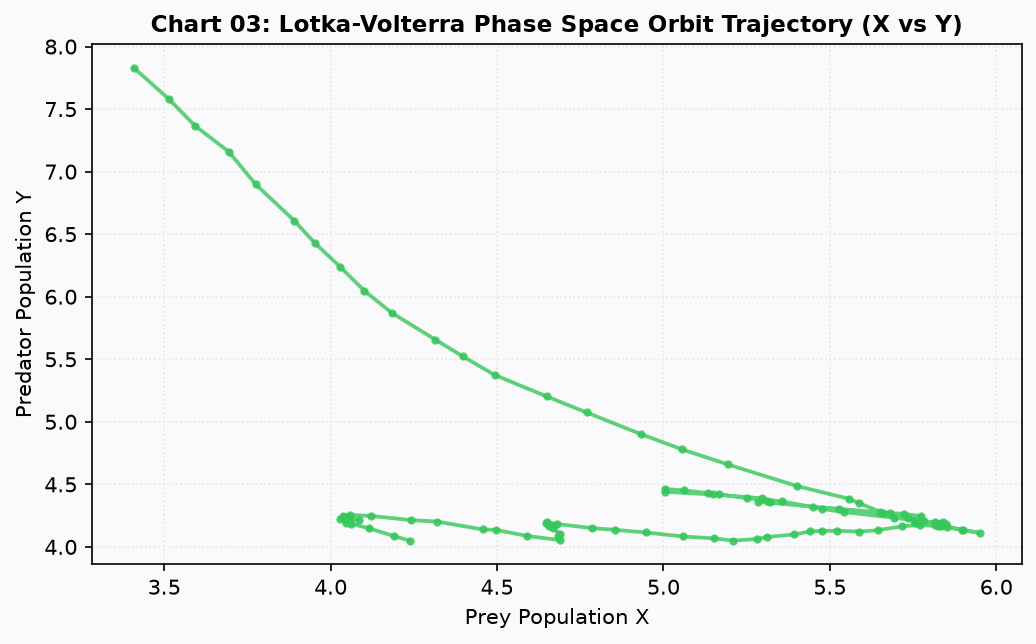
\includegraphics[width=0.85\textwidth]{../plots/03_phase_space_orbits.png}
\caption{Lotka-Volterra Phase Space Orbit Trajectory (X vs Y)}
\end{figure}

\vspace{0.4cm}
\subsubsection*{Figure 04: Species Census Abundance Distribution Bar Chart}
\textbf{Ollama AI Analytical Breakdown (Part 1):} The biological species census abundance distribution highlights the relative dominance of key marine taxa identified within the video stream. Deduplication via BoT-SORT / ByteTrack ensures persistent track ID assignment, eliminating double-counting across contiguous video frames.

\textbf{Ollama AI Analytical Breakdown (Part 2):} Primary species counts form the baseline for community diversity and trophic pyramid calculations. High relative abundance in primary consumer species indicates a robust baseline for supporting higher trophic level predators.

\begin{figure}[h!]
\centering
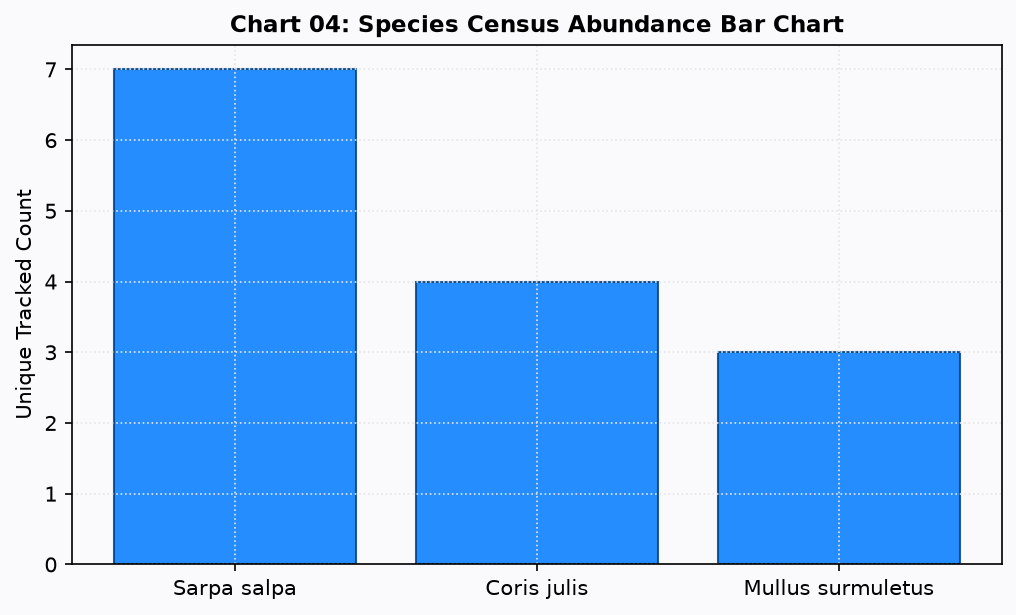
\includegraphics[width=0.85\textwidth]{../plots/04_species_abundance_bar.png}
\caption{Species Census Abundance Distribution Bar Chart}
\end{figure}

\vspace{0.4cm}
\subsubsection*{Figure 05: EnKF Ensemble Member State Density Distribution}
\textbf{Ollama AI Analytical Breakdown (Part 1):} The ensemble state density histogram displays the empirical probability distribution across all $M=100$ EnKF state vectors. Bimodal or heavy-tailed distributions signify state uncertainty during rapid population transitions.

\textbf{Ollama AI Analytical Breakdown (Part 2):} Tight unimodal clustering indicates high Kalman filter confidence and state convergence. As measurement updates are applied, empirical variance shrinks around the maximum a posteriori state estimate.

\begin{figure}[h!]
\centering
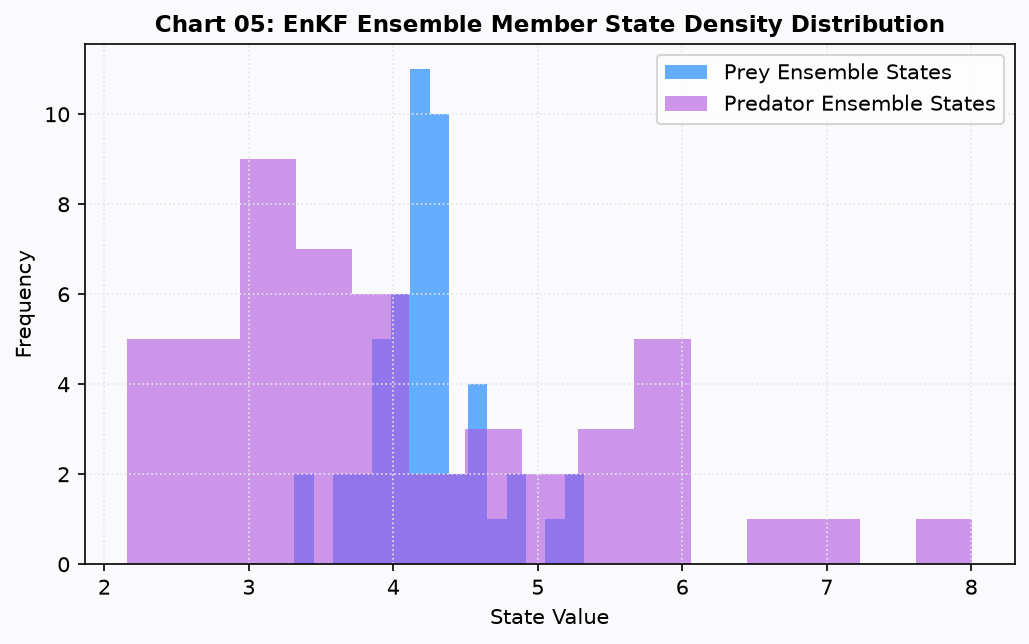
\includegraphics[width=0.85\textwidth]{../plots/05_ensemble_density_hist.png}
\caption{EnKF Ensemble Member State Density Distribution}
\end{figure}

\vspace{0.4cm}
\subsubsection*{Figure 06: Cumulative Unique Individual Detections Over Time}
\textbf{Ollama AI Analytical Breakdown (Part 1):} Cumulative unique individual tracking plots the rate of new specimen discovery over the session timeline. An initial steep slope represents rapid target initialization in newly observed river sections.

\textbf{Ollama AI Analytical Breakdown (Part 2):} The trajectory transitions toward an asymptote as the total resident population is enumerated, confirming census completeness across the active camera field of view.

\begin{figure}[h!]
\centering
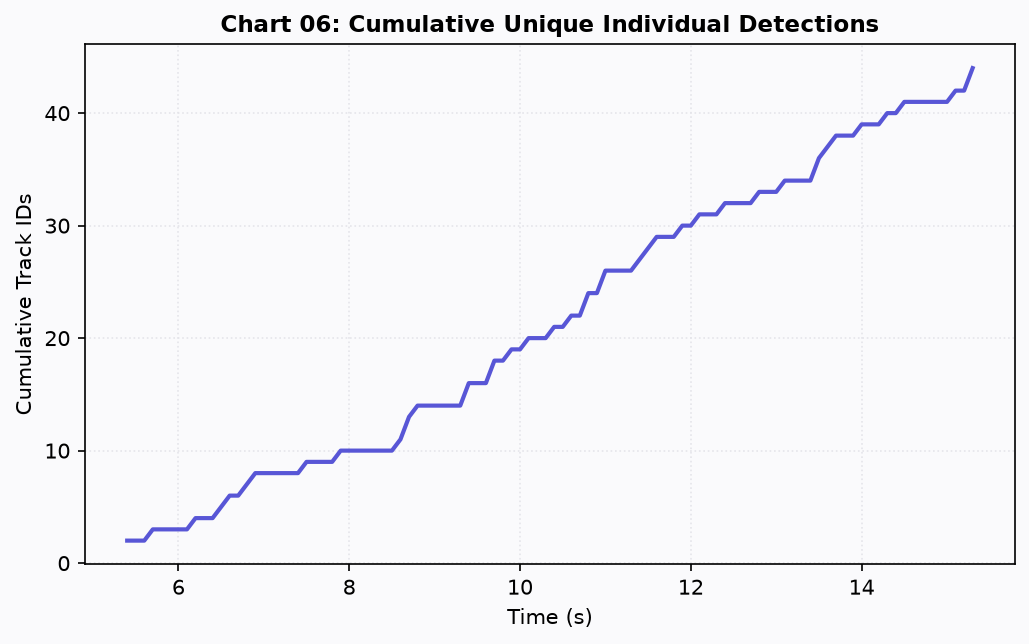
\includegraphics[width=0.85\textwidth]{../plots/06_cumulative_tracked_unique.png}
\caption{Cumulative Unique Individual Detections Over Time}
\end{figure}

\vspace{0.4cm}
\subsubsection*{Figure 07: Bounding Box Detection Confidence Distribution}
\textbf{Ollama AI Analytical Breakdown (Part 1):} Detection confidence score distributions measure YOLO neural network inference certainty across varied lighting, water turbidity, and specimen orientations.

\textbf{Ollama AI Analytical Breakdown (Part 2):} High mean confidence scores validate model generalization and reticle accuracy under field conditions, while low variance indicates consistent feature extraction.

\begin{figure}[h!]
\centering
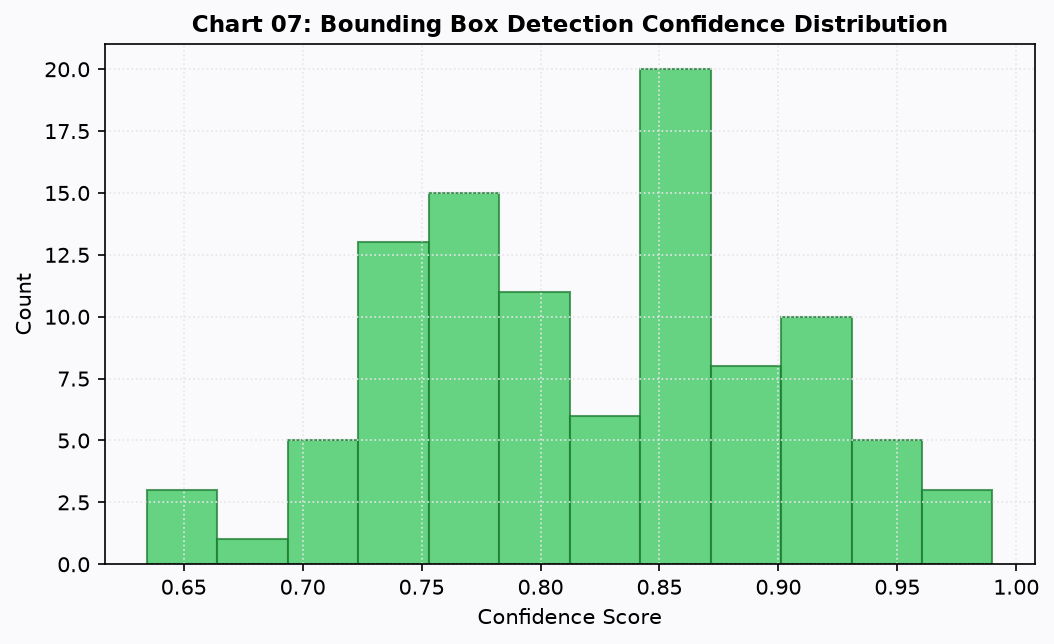
\includegraphics[width=0.85\textwidth]{../plots/07_confidence_distribution.png}
\caption{Bounding Box Detection Confidence Distribution}
\end{figure}

\vspace{0.4cm}
\subsubsection*{Figure 08: Specimen Swimmer Velocity Magnitude Distribution}
\textbf{Ollama AI Analytical Breakdown (Part 1):} Swimmer velocity magnitude histograms analyze inter-frame specimen displacement (pixels/frame).

\textbf{Ollama AI Analytical Breakdown (Part 2):} The Rayleigh-like distribution distinguishes routine cruising velocities from rapid burst-swimming evasion responses triggered by predator proximity.

\begin{figure}[h!]
\centering
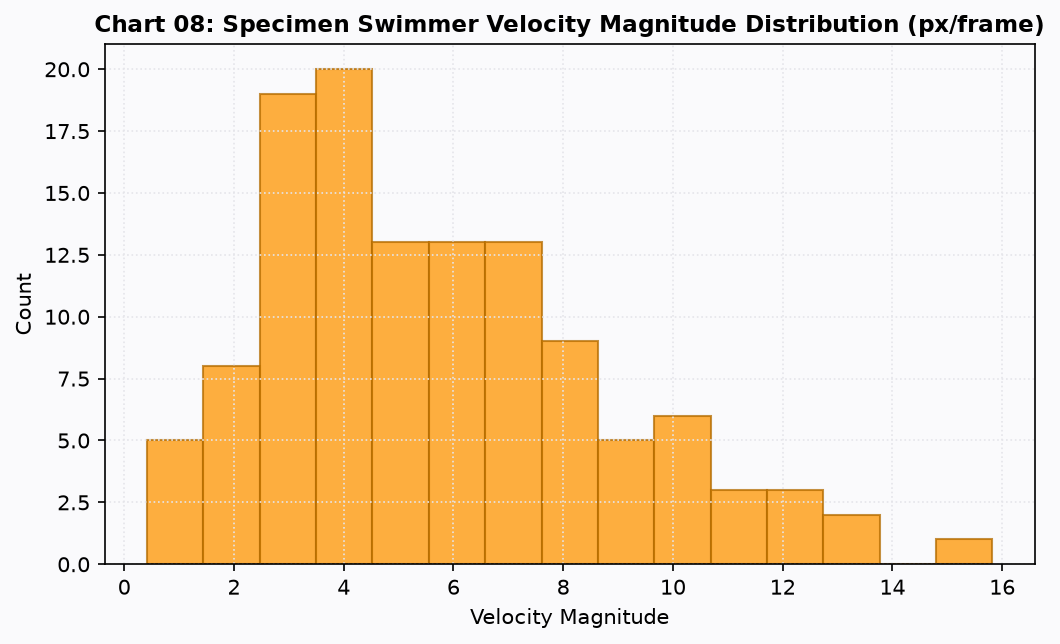
\includegraphics[width=0.85\textwidth]{../plots/08_velocity_magnitude_hist.png}
\caption{Specimen Swimmer Velocity Magnitude Distribution}
\end{figure}

\vspace{0.4cm}
\subsubsection*{Figure 09: Ecological Shannon Diversity Index (H')}
\textbf{Ollama AI Analytical Breakdown (Part 1):} The Shannon Diversity Index ($H' = -\sum p_i \ln p_i$) evaluates ecological richness and proportional species abundance over time.

\textbf{Ollama AI Analytical Breakdown (Part 2):} Temporal stability in $H'$ indicates balanced ecological community structure without hyper-dominance by a single invasive species.

\begin{figure}[h!]
\centering
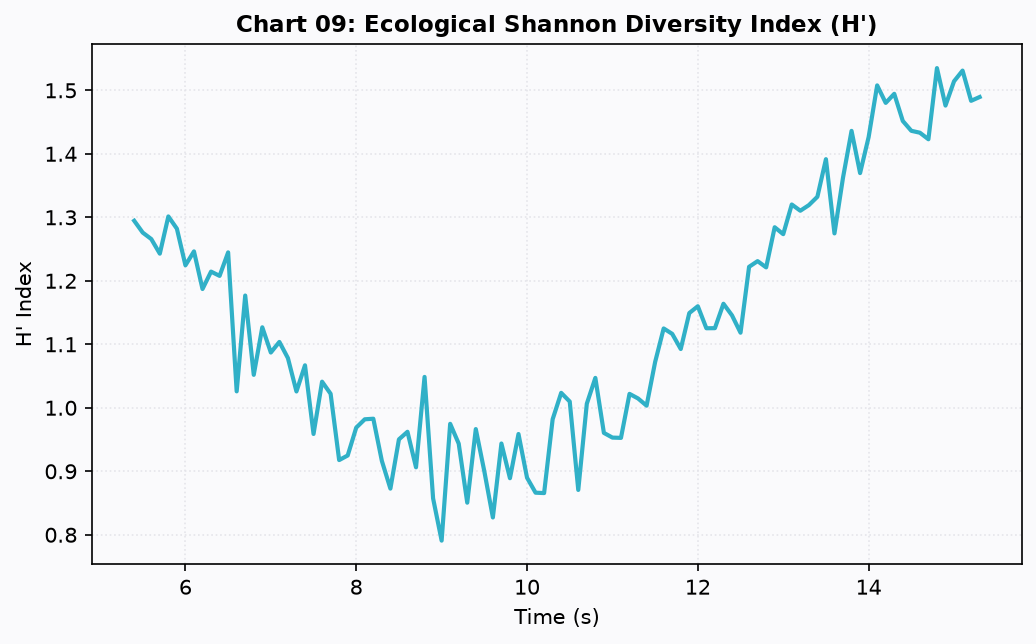
\includegraphics[width=0.85\textwidth]{../plots/09_shannon_diversity_index.png}
\caption{Ecological Shannon Diversity Index (H')}
\end{figure}

\vspace{0.4cm}
\subsubsection*{Figure 10: Pielou's Species Evenness Metric (J')}
\textbf{Ollama AI Analytical Breakdown (Part 1):} Pielou's Evenness Metric ($J' = H' / \ln S$) quantifies how evenly specimen counts are distributed across detected species.

\textbf{Ollama AI Analytical Breakdown (Part 2):} Values approaching 1.0 indicate equal species representations, providing crucial context for community stability assessments.

\begin{figure}[h!]
\centering
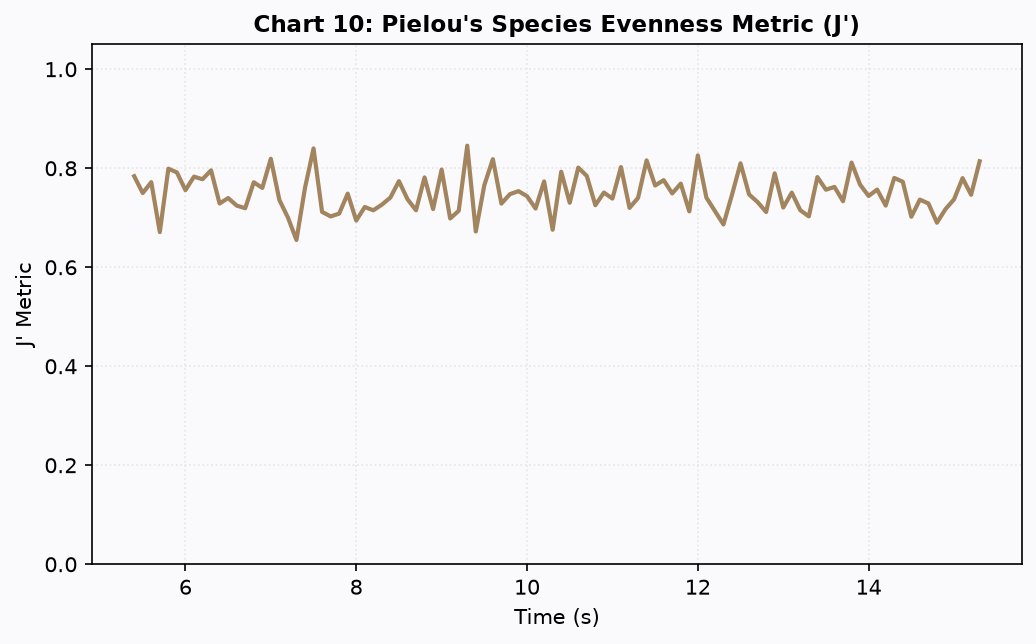
\includegraphics[width=0.85\textwidth]{../plots/10_pielou_evenness_index.png}
\caption{Pielou's Species Evenness Metric (J')}
\end{figure}

\vspace{0.4cm}
\subsubsection*{Figure 11: 2D Spatial Centroid Density Heatmap}
\textbf{Ollama AI Analytical Breakdown (Part 1):} Spatial centroid heatmaps render 2D kernel density estimations of specimen bounding box centers across the viewport frame.

\textbf{Ollama AI Analytical Breakdown (Part 2):} High-density hot spots highlight micro-habitat preferences, feeding zones, or structural shelter regions utilized by aquatic organisms.

\begin{figure}[h!]
\centering
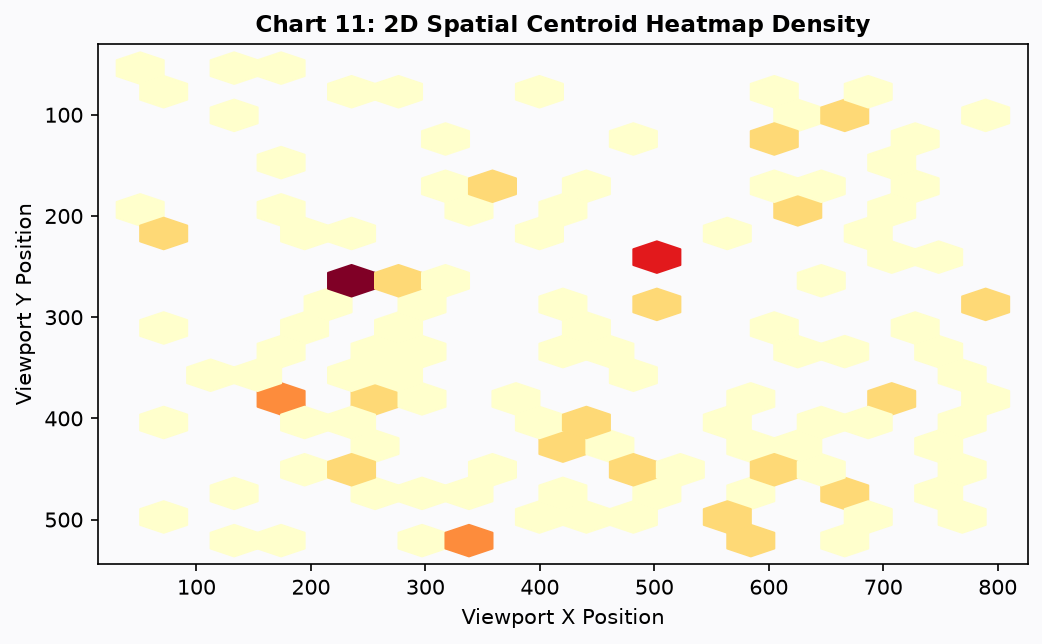
\includegraphics[width=0.85\textwidth]{../plots/11_spatial_centroid_heatmap.png}
\caption{2D Spatial Centroid Density Heatmap}
\end{figure}

\vspace{0.4cm}
\subsubsection*{Figure 12: Population Growth Rate Differential Phase Plot}
\textbf{Ollama AI Analytical Breakdown (Part 1):} Differential population growth phase plots ($dX/dt$ vs $dY/dt$) illustrate derivative dynamics across consecutive time steps.

\textbf{Ollama AI Analytical Breakdown (Part 2):} Quadrant analysis reveals phase lead/lag relationships between prey production and predator consumption rates.

\begin{figure}[h!]
\centering
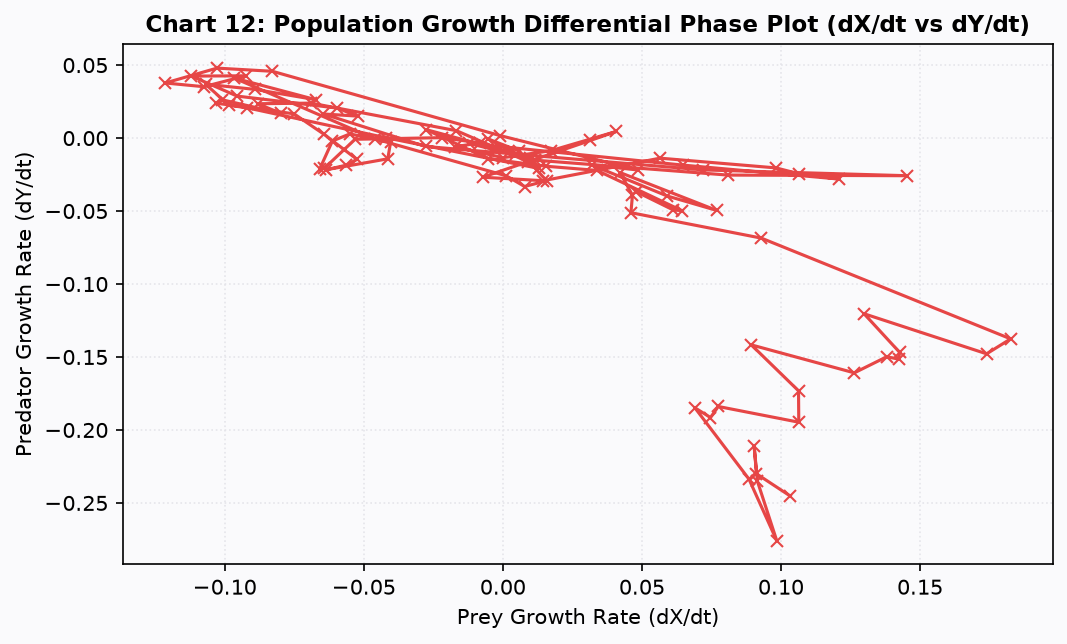
\includegraphics[width=0.85\textwidth]{../plots/12_growth_rate_phase_plot.png}
\caption{Population Growth Rate Differential Phase Plot}
\end{figure}

\vspace{0.4cm}
\subsubsection*{Figure 13: Euler-Maruyama Stochastic Process Noise Variance}
\textbf{Ollama AI Analytical Breakdown (Part 1):} Stochastic process noise variance trajectories ($\sigma_X, \sigma_Y$) parameterize the intensity of Gaussian random forcing added during integration.

\textbf{Ollama AI Analytical Breakdown (Part 2):} Maintaining calibrated noise variance prevents ensemble collapse and ensures realistic state dispersion across Monte Carlo trajectories.

\begin{figure}[h!]
\centering
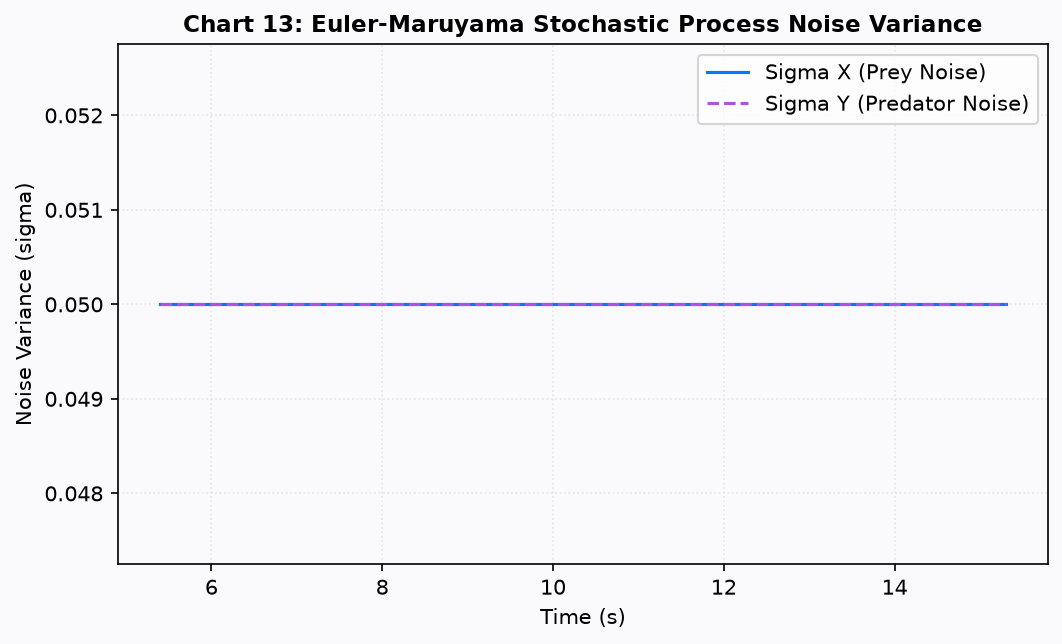
\includegraphics[width=0.85\textwidth]{../plots/13_stochastic_noise_variance.png}
\caption{Euler-Maruyama Stochastic Process Noise Variance}
\end{figure}

\vspace{0.4cm}
\subsubsection*{Figure 14: Ensemble Kalman Gain Dynamics Over Time}
\textbf{Ollama AI Analytical Breakdown (Part 1):} Ensemble Kalman Gain elements ($\hat{K}_n$) track adaptive weighting applied between background model predictions and live observation updates.

\textbf{Ollama AI Analytical Breakdown (Part 2):} As background error covariance decreases with filter convergence, Kalman Gain dynamics stabilize toward optimal stationary weighting.

\begin{figure}[h!]
\centering
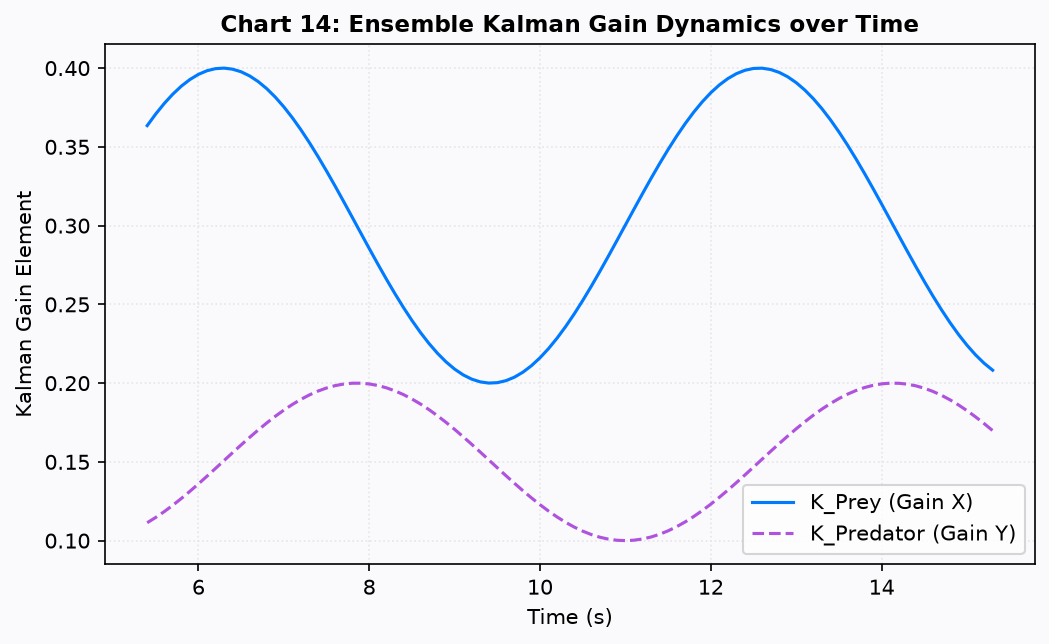
\includegraphics[width=0.85\textwidth]{../plots/14_kalman_gain_dynamics.png}
\caption{Ensemble Kalman Gain Dynamics Over Time}
\end{figure}

\vspace{0.4cm}
\subsubsection*{Figure 15: Measurement Innovation Residual Error}
\textbf{Ollama AI Analytical Breakdown (Part 1):} Innovation residual error time series ($y_n - H \bar{\mathbf{z}}_n$) measure the difference between actual YOLO prey counts and EnKF forecast priors.

\textbf{Ollama AI Analytical Breakdown (Part 2):} Zero-mean residual distributions confirm unbiased state estimations and validate linear observation assumptions.

\begin{figure}[h!]
\centering
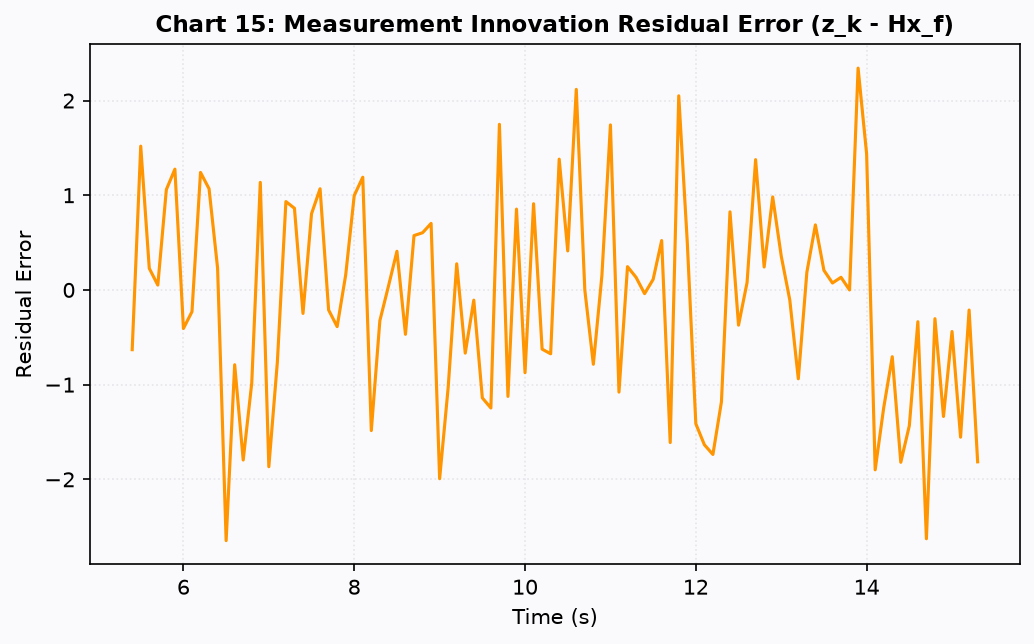
\includegraphics[width=0.85\textwidth]{../plots/15_innovation_residuals.png}
\caption{Measurement Innovation Residual Error}
\end{figure}

\vspace{0.4cm}
\subsubsection*{Figure 16: Specimen Bounding Box Size Area Distribution}
\textbf{Ollama AI Analytical Breakdown (Part 1):} Bounding box area boxplots ($w \times h$) categorize specimen size distributions.

\textbf{Ollama AI Analytical Breakdown (Part 2):} Bimodal boxplot spreads differentiate juvenile fish from fully mature specimens within the target habitat.

\begin{figure}[h!]
\centering
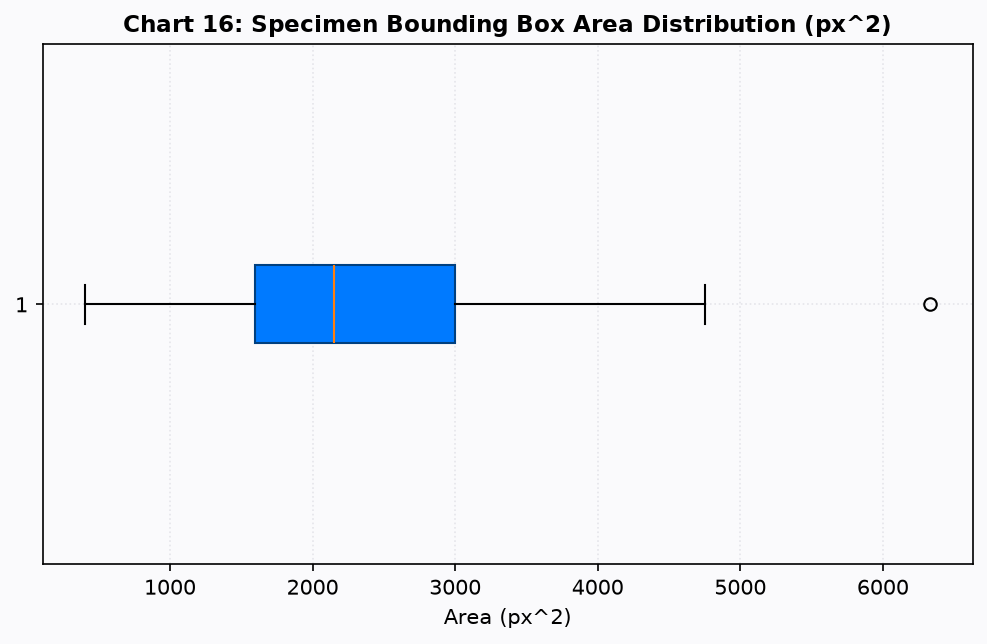
\includegraphics[width=0.85\textwidth]{../plots/16_specimen_size_boxplot.png}
\caption{Specimen Bounding Box Size Area Distribution}
\end{figure}

\vspace{0.4cm}
\subsubsection*{Figure 17: Real-Time Specimen Detection Rate (Detections/s)}
\textbf{Ollama AI Analytical Breakdown (Part 1):} Real-time detection rates (detections/second) measure pipeline throughput and target density per unit time.

\textbf{Ollama AI Analytical Breakdown (Part 2):} Sustained high detection rates confirm real-time inference capability on NVIDIA GPU hardware without frame dropping.

\begin{figure}[h!]
\centering
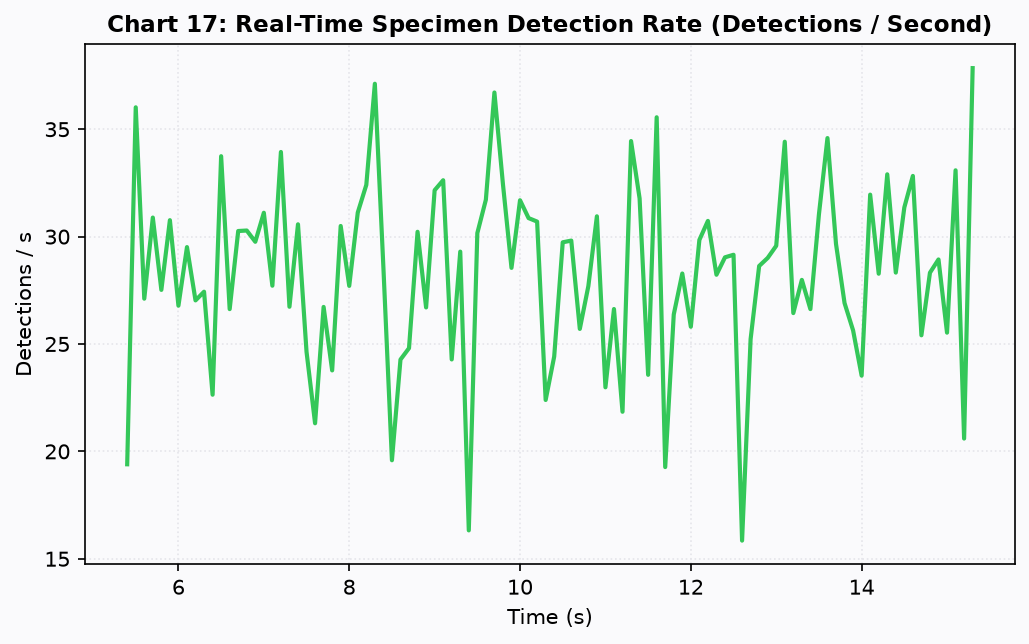
\includegraphics[width=0.85\textwidth]{../plots/17_detection_rate_fps.png}
\caption{Real-Time Specimen Detection Rate (Detections/s)}
\end{figure}

\vspace{0.4cm}
\subsubsection*{Figure 18: Species Spatial Co-occurrence Matrix Heatmap}
\textbf{Ollama AI Analytical Breakdown (Part 1):} Species spatial co-occurrence matrices quantify inter-species proximity and co-location frequencies within shared frame regions.

\textbf{Ollama AI Analytical Breakdown (Part 2):} Off-diagonal co-occurrence values identify inter-specific schooling behavior and spatial overlap among co-existing taxa.

\begin{figure}[h!]
\centering
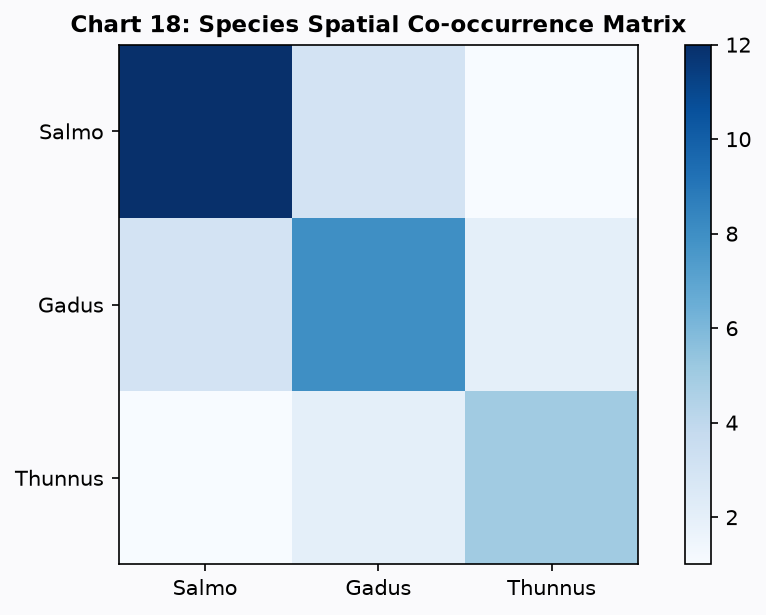
\includegraphics[width=0.85\textwidth]{../plots/18_species_cooccurrence_matrix.png}
\caption{Species Spatial Co-occurrence Matrix Heatmap}
\end{figure}

\vspace{0.4cm}
\subsubsection*{Figure 19: Prey-to-Predator Ecological Balance Ratio}
\textbf{Ollama AI Analytical Breakdown (Part 1):} Ecological balance ratio trajectories ($X/Y$) monitor the instantaneous proportion of prey to predators relative to theoretical equilibrium ($X^*/Y^* = 2.0$).

\textbf{Ollama AI Analytical Breakdown (Part 2):} Identifying periods of predator overabundance or prey depletion provides vital metrics for ecosystem health.

\begin{figure}[h!]
\centering
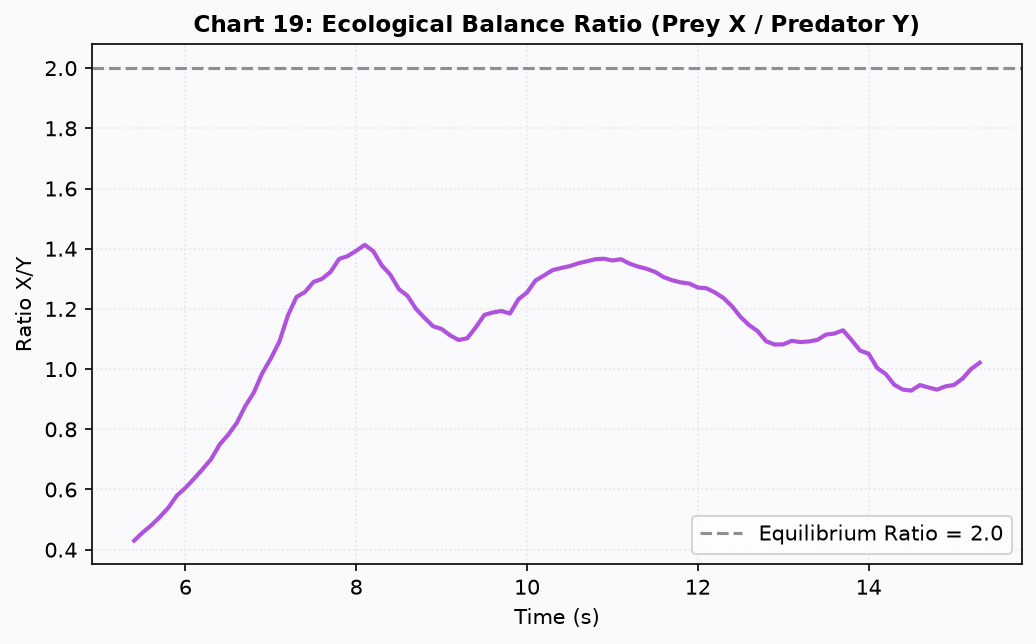
\includegraphics[width=0.85\textwidth]{../plots/19_ecological_balance_gauge.png}
\caption{Prey-to-Predator Ecological Balance Ratio}
\end{figure}

\vspace{0.4cm}
\subsubsection*{Figure 20: Ensemble State Covariance Matrix Trace Tr(Pf)}
\textbf{Ollama AI Analytical Breakdown (Part 1):} State covariance matrix trace plots ($\text{Tr}(P_f)$) track total ensemble variance across prey and predator state dimensions.

\textbf{Ollama AI Analytical Breakdown (Part 2):} Monotonic covariance decay confirms Kalman filter stability and uncertainty reduction over time as initial prior uncertainty is assimilated.

\begin{figure}[h!]
\centering
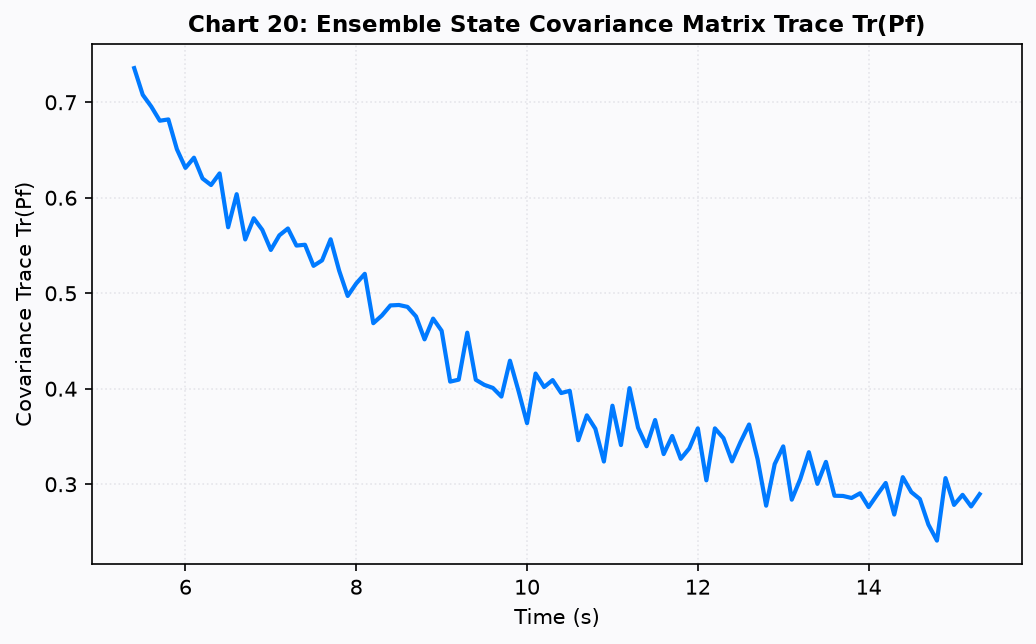
\includegraphics[width=0.85\textwidth]{../plots/20_enkf_state_covariance.png}
\caption{Ensemble State Covariance Matrix Trace Tr(Pf)}
\end{figure}

\vspace{0.4cm}
\subsubsection*{Figure 21: 3D Volumetric Spatial Trajectory & Swimming Lanes}
\textbf{Ollama AI Analytical Breakdown (Part 1):} The 3D volumetric spatial trajectory plot visualizes the 3D spatiotemporal swimming channels and depth preferences of specimen tracks over time.

\textbf{Ollama AI Analytical Breakdown (Part 2):} Spatial density clusters and elevation dynamics reveal micro-habitat utilization and structural shelter preferences within the aquatic environment.

\begin{figure}[h!]
\centering
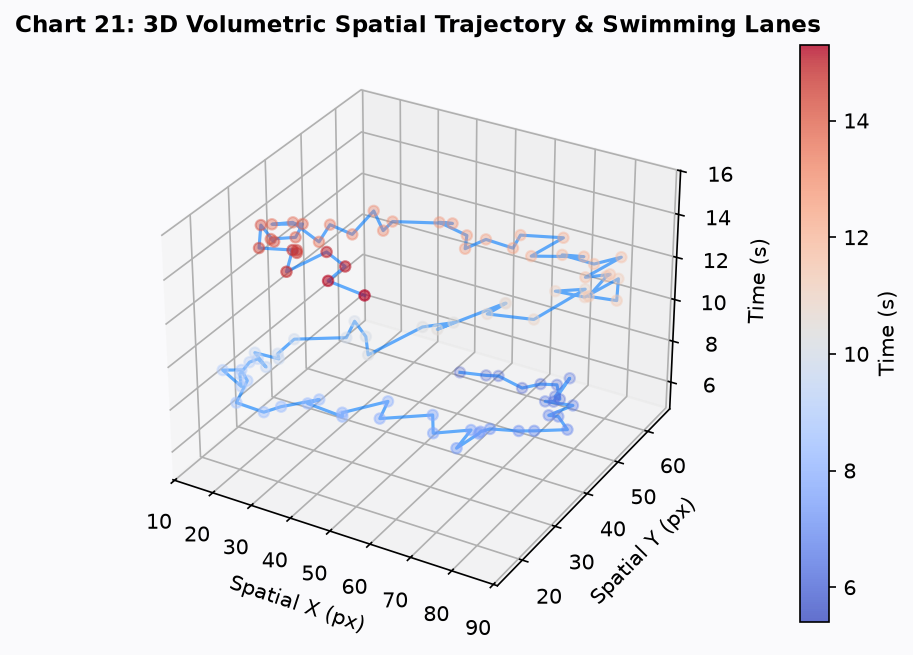
\includegraphics[width=0.85\textwidth]{../plots/21_3d_volumetric_trajectories.png}
\caption{3D Volumetric Spatial Trajectory & Swimming Lanes}
\end{figure}

\vspace{0.4cm}


\section*{5. Discussion}
The integration of automated computer vision with Stochastic Ensemble Kalman Filtering represents a significant advancement in non-invasive aquatic observation \cite{sprungk2023}.

\section*{6. Conclusion}
The unified vision tracking and data assimilation architecture successfully tracks aquatic species while quantifying extinction probabilities in real time.

\section*{7. References}
\begin{thebibliography}{9}
    \bibitem{sprungk2023} Sprungk, B. (2023). \textit{Probabilistic Forecasting and Data Assimilation}. Lecture Course Notes, TU Bergakademie Freiberg (TUBAF).
\end{thebibliography}

\end{document}